\section{GraphBLAS Operations}
\label{Sec:Operations}

The GraphBLAS operations are defined in the GraphBLAS math specification and summarized in 
Table~\ref{Tab:GraphBLASOps}.   In addition to methods that implement these
fundamental GraphBLAS operations, we support a number of variants that have been 
found to be especially useful in algorithm development.
A flowchart of the overall behavior of a GraphBLAS operation is shown 
in Figure~\ref{Fig:mxmFlowchart}.


\begin{table}[tb]
\hrule
\begin{center}
\caption{A mathematical notation for the fundamental GraphBLAS operations 
supported in this specification.  Input matrices $\matrix{A}$ and $\matrix{B}$ 
may be optionally transposed (not shown). Use of an optional accumulate with 
existing values in the output object is indicated with $\odot$.  Use of optional write 
masks and replace flags are indicated as $\matrix{C}\langle\matrix{M},z\rangle$ 
when applied to the output matrix, $\matrix{C}$.  The mask controls which values 
resulting from the operation on the right-hand side are written into the output 
object (complement and structure flags are not shown).  The ``replace" 
option, indicated by specifying the $z$ flag, means that all values in the 
output object are removed prior to assignment. If ``replace" is not specifed, 
only the values/locations computed on the right-hand side and allowed by the 
mask will be written to the output (``merge" mode).}
\label{Tab:GraphBLASOps}
~\\
\newcommand{\odotsp}{\hspace{-0.2cm}\odot\hspace{-0.18cm}}
\begin{tabular}{l|rcrcl}
{\sf Operation Name} & \multicolumn{5}{c}{Mathematical Notation}  \\
\hline
{\sf mxm}          & $\matrix{C}\langle\matrix{M},z\rangle$ & $=$ & $\matrix{C}$ & $\odotsp$ & $\matrix{A} \oplus.\otimes \matrix{B}$  \\
{\sf mxv}          & $\vector{w}\langle\vector{m},z\rangle$ & $=$ & $\vector{w}$ & $\odotsp$ & $\matrix{A} \oplus.\otimes \vector{u}$  \\
{\sf vxm}          & $\vector{w}^T\langle\vector{m}^T,z\rangle$ & $=$ & \hspace{-0.18cm}$\vector{w}^T$ & $\odotsp$ & $\vector{u}^T \oplus.\otimes \matrix{A}$  \\
{\sf eWiseMult}    & $\matrix{C}\langle\matrix{M},z\rangle$ & $=$ & $\matrix{C}$ & $\odotsp$ & $\matrix{A} \otimes \matrix{B}$  \\
                   & $\vector{w}\langle\matrix{m},z\rangle$ & $=$ & $\vector{w}$ & $\odotsp$ & $\vector{u} \otimes \vector{v}$  \\
{\sf eWiseAdd}     & $\matrix{C}\langle\matrix{M},z\rangle$ & $=$ & $\matrix{C}$ & $\odotsp$ & $\matrix{A} \oplus  \matrix{B}$  \\
                   & $\vector{w}\langle\matrix{m},z\rangle$ & $=$ & $\vector{w}$ & $\odotsp$ & $\vector{u} \oplus \vector{v}$  \\
{\sf reduce} (row) & $\vector{w}\langle\vector{m},z\rangle$ & $=$ & $\vector{w}$ & $\odotsp$ & $\left[\oplus_j\matrix{A}(:,j)\right]$  \\
{\sf reduce} (scalar) & $s$ & $=$ & $s$ & $\odotsp$ & $\left[\oplus_{i,j}\matrix{A}(i,j) \right]$  \\
                      & $s$ & $=$ & $s$ & $\odotsp$ & $\left[\oplus_i\matrix{u}(i) \right]$  \\
{\sf apply}        & $\matrix{C}\langle\matrix{M},z\rangle$ & $=$ & $\matrix{C}$ & $\odotsp$ & $f_u(\matrix{A})$ \\
                   & $\vector{w}\langle\matrix{m},z\rangle$ & $=$ & $\vector{w}$ & $\odotsp$ & $f_u(\vector{u} )$  \\
{\sf transpose}    & $\matrix{C}\langle\matrix{M},z\rangle$ & $=$ & $\matrix{C}$ & $\odotsp$ & $\matrix{A}^T$ \\
{\sf extract}      & $\matrix{C}\langle\matrix{M},z\rangle$ & $=$ & $\matrix{C}$ & $\odotsp$ & $\matrix{A}(\grbarray{i},\grbarray{j})$ \\
                   & $\vector{w}\langle\matrix{m},z\rangle$ & $=$ & $\vector{w}$ & $\odotsp$ & $\vector{u}(\grbarray{i})$ \\
%{\sf extract} (column) & $\matrix{w}\langle\vector{m},z\rangle$ & $=$ & $\matrix{w}$ & $\odotsp$ & $\matrix{A}(\grbarray{i}, j)$ \\
{\sf assign}       & $\matrix{C}\langle\matrix{M},z\rangle(\grbarray{i},\grbarray{j})$ & $=$ & $\matrix{C}(\grbarray{i},\grbarray{j})$ & $\odotsp$ & $\matrix{A}$ \\
                   & $\vector{w}\langle\vector{m},z\rangle(\grbarray{i})$ & $=$ & $\vector{w}(\grbarray{i})$ & $\odotsp$ & $\matrix{u}$ \\
%& & & \\
%& \multicolumn{3}{c}{Input/Output Operations} \\
%{\sf Matrix\_build}  & $\matrix{C}$ & $=$ & $\mathbb{S}^{m\times n}(\grbarray{i},\grbarray{j},\grbarray{v},\oplus_{dup})$ \\
%{\sf Vector\_build}  & $\vector{w}$ & $=$ & $\mathbb{S}^{n}(\grbarray{i},\grbarray{v},\oplus_{dup})$ \\
%{\sf Matrix\_extractTuples} & $(\grbarray{i},\grbarray{j},\grbarray{v})$ & $=$ & $\matrix{A}$ \\
%{\sf Vector\_extractTuples} & $(\grbarray{i},\grbarray{v})$ & $=$ & $\matrix{u}$ \\
\end{tabular}
\end{center}
\hrule
\end{table}

\paragraph{Domains and Casting}

A GraphBLAS operation is only valid when the domains of the GraphBLAS objects are
mathematically consistent.  The C programming language defines implicit casts 
between built-in data types.  For example, {\sf float}s, {\sf double}s, and {\sf int}s can be 
freely mixed according to the rules defined for implicit casts.  It is the 
responsibility of the user to assure that these casts are appropriate for the 
algorithm in question.  For example, a cast to {\sf int} implies truncation of a floating 
point type.  Depending on the operation, this truncation error could lead to
erroneous results.  Furthermore, casting a wider type onto a narrower type can lead 
to overflow errors.  The GraphBLAS operations do not attempt to protect a user from 
these sorts of errors.

When user-define types are involved, however, GraphBLAS requires strict equivalence
between types and no casting is supported.  If GraphBLAS detects these mismatches,
it will return a domain mismatch error.

\begin{figure}
    \hrule
    \begin{center}
        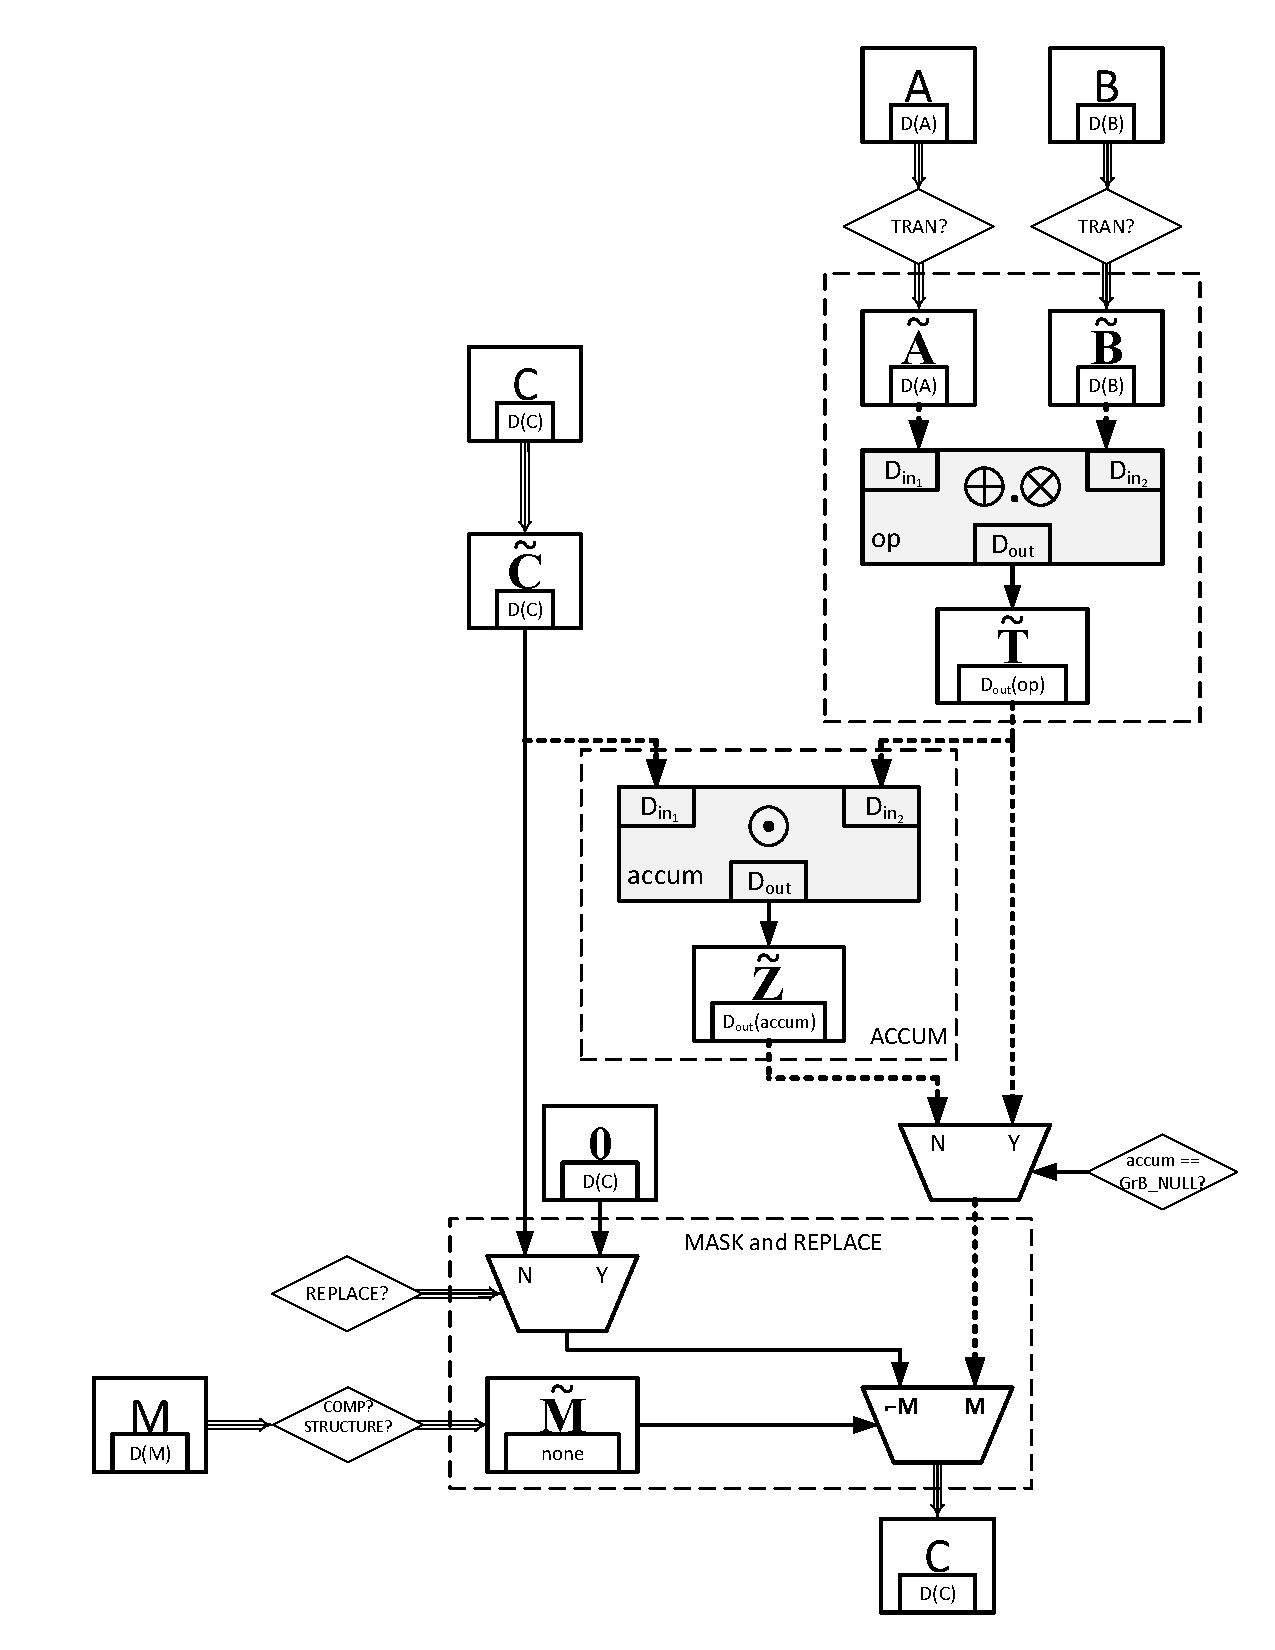
\includegraphics[width=5.5in]{mxm_operation_flowchart_1_3d.pdf}
    \end{center}
    \caption{Flowchart for the GraphBLAS operations. Although shown specifically for
	the {\sf mxm} operation, many elements are common to all operations: such as the 
	``{\sf ACCUM}'' and ``{\sf MASK and REPLACE}'' blocks.  The "triple" arrows 
    ($\Rrightarrow$) denote where ``as if copy'' takes place (including both 
    collections and descriptor settings).  The bold, dotted arrows indicate
    where casting may occur between different domains. \scott{STRUCTURE\_ONLY changes.}}
    \label{Fig:mxmFlowchart}
    \hrule
\end{figure}

\paragraph{Dimensions and Transposes}

GraphBLAS operations also make assumptions about the numbers of dimensions and 
sizes of vectors and matrices in an operation.   An operation will test these 
sizes and report an error if they are not \emph{shape compatible}.  For example, when multiplying 
two matrices, $\matrix{C} = \matrix{A} \times \matrix{B}$, the number of rows of 
$\matrix{C}$ must equal the number of rows of $\matrix{A}$, the number of columns 
of $\matrix{A}$ must match the number of rows of $\matrix{B}$, and the number of 
columns of $\matrix{C}$ must match then number of columns of $\matrix{B}$.  This 
is the behavior expected given the mathematical definition of the operations.   

For most of the GraphBLAS operations involving matrices, an optional descriptor 
can modify the matrix associated with an input GraphBLAS matrix object.  For 
example, if an input matrix is an argument to a GraphBLAS operation and the 
associated descriptor indicates the transpose option, then the operation occurs 
as if on the transposed matrix.  In this case, the relationships between the 
sizes in each dimension shift in the mathematically expected way. 

\paragraph{Masks: Structure-only, Complement, and Replace}

When a GraphBLAS operation supports the use of an optional mask, that mask is
specified through a GraphBLAS vector (for one-dimensional masks) or
a GraphBLAS matrix (for two-dimensional masks).  When a mask is used and the 
{\tt GrB\_STRUCTURE} descriptor value is not set, it is applied to the result 
from the operation wherever the stored values in the mask evaluate to true.  If
the {\tt GrB\_STRUCTURE} descriptor is set, the mask is applied to the result
from the operation wherever the mask as a stored value (regardless of that value).
Wherever the mask is applied, the result from the operation is either assigned 
to the provided output matrix/vector or, if a binary accumulation operation is 
provided, the result is accumulated into the corresponding elements of the provided 
output matrix/vector. \scott{STRUCTURE\_ONLY changes.}

Given a GraphBLAS vector $\vector{v} = \langle D,N, \{ (i,v_i) \} \rangle$, a
one-dimensional mask is derived for use in the operation as follows:
\[
\vector{m} = 
\begin{cases}
\langle N, \{ \mathbf{ind}(\vector{v}) \} \rangle, & \mbox{if {\tt GrB\_STRUCTURE} is specified,} \\
\langle N, \{ i : \mbox{\tt (bool)}v_i = \true \} \rangle, & \mbox{otherwise}
\end{cases}
\]
where {\tt (bool)}$v_i$ denotes casting the value $v_i$ to a Boolean value (\true\ or \false).
Likewise, given a GraphBLAS matrix $\matrix{A} = \langle D, M, N, \{ (i,j,A_{ij}) \} \rangle$,
a two-dimensional mask is derived for use in the operation as follows:
\[
\matrix{M} = 
\begin{cases}
\langle M,N, \{ \mathbf{ind}(\matrix{A}) \} \rangle, & \mbox{if {\tt GrB\_STRUCTURE} is specified,} \\
\langle M,N, \{ (i,j) : \mbox{\tt (bool)}A_{ij} = \true \} \rangle, & \mbox{otherwise}
\end{cases}
\]
where {\tt (bool)}$A_{ij}$ denotes casting the value $A_{ij}$ to a Boolean value. 
(\true\ or \false)\scott{STRUCTURE\_ONLY changes}

In both the one- and two-dimensional cases, the mask may also have a subsequent 
complement operation applied ($\S$~\ref{Sec:Masks}) as specified in the 
descriptor, before a final mask is generated for use in the operation.

When the descriptor of an operation with a mask has specified that 
the {\sf GrB\_REPLACE} value is to be applied to the output ({\sf GrB\_OUTP}),
then anywhere the mask is not {\sf true}, the corresponding location in
the output is cleared.


\paragraph{Invalid and uninitialized objects}

Upon entering a GraphBLAS operation, the first step is a check that all
objects are valid and initialized. (Optional parameters can be set to {\sf
GrB\_NULL}, which always counts as a valid object.)  An invalid object is
one that could not be computed due to some previous execution error. An
unitialized ojbect is one that has not yet been created by a corresponding
{\sf new} or {\sf dup} method.  Appropriate error codes are returned if
an object is not initialized ({\sf GrB\_UNINITIALIZED\_OBJECT}) or invalid
({\sf GrB\_INVALID\_OBJECT}).

To support the detection of as many cases of uninitialized objects as possible,
it is strongly recommended to initialize all GraphBLAS objects to
the predefined value {\sf GrB\_INVALID\_HANDLE} at the point of their declaration,
as shown in the following examples:

\begin{verbatim}
        GrB_Type        type = GrB_INVALID_HANDLE;
        GrB_Semiring    semiring = GrB_INVALID_HANDLE;
        GrB_Matrix      matrix = GrB_INVALID_HANDLE;
\end{verbatim}

\paragraph{Compliance}

We follow a \emph{prescriptive} approach to the definition of the semantics
of GraphBLAS operations. That is, for each operation we give a recipe for
producing its outcome.
It should be understood that any implementation that produces the same outcome,
and follows the GraphBLAS execution model (\S~\ref{Sec:ExecutionModel}) and
error model (\S~\ref{Sec:ErrorModel}), is a conforming implementation.
